\documentclass[a4wide, 11pt]{article}
\usepackage{a4, fullpage}
\setlength{\parskip}{0.2cm}
\setlength{\parindent}{0cm}
\usepackage[hmargin=2.2cm,vmargin=2.3cm]{geometry}
\usepackage{url}
\usepackage{hyperref}
\usepackage{breakurl}

% This is the preamble section where you can include extra packages etc.

\ifx\pdftexversion\undefined
\usepackage[dvips]{graphicx}
\else
\usepackage[pdftex]{graphicx}
\DeclareGraphicsRule{*}{mps}{*}{}
\fi

\begin{document}

\title{Software Engineering Coursework \\ Design and Implementation of Multiplayer Othello}

\author{Michal Srb and Thomas Rooney}

\date{\today}         % inserts today's date

\maketitle            % generates the title from the data above

\section{Introduction}

The task that we have been given is to design and implement a computer-based version of Othello, that is playable between at least two human players.

To implement this, we have decided to leverage web technologies to build a webpage, that when loaded, provides the player with a UI for a multiplayer lobby, through which the players can challenge one another and play a game of Reversi.

To focus our design efforts, we decided to utilise the Test Driven Development style through the following workflow:
\begin{enumerate}
\item Writing Calling Code
\item Write a shell implementation of the feature, just enough such that it compiles
\item Use Test Driven Development:- writing tests for the feature using the methods defined above; defining the methods such that tests pass \ldots
\item End up with finished, and tested feature
\end{enumerate}

In designing each component, we also attempted to adhere to \texttt{Object Oriented} principles, wherby the number of public methods in each class is minimized to the bare requirement of the features that are inherently necessary to the functionality of the object. This leads to a clean, and simple design.

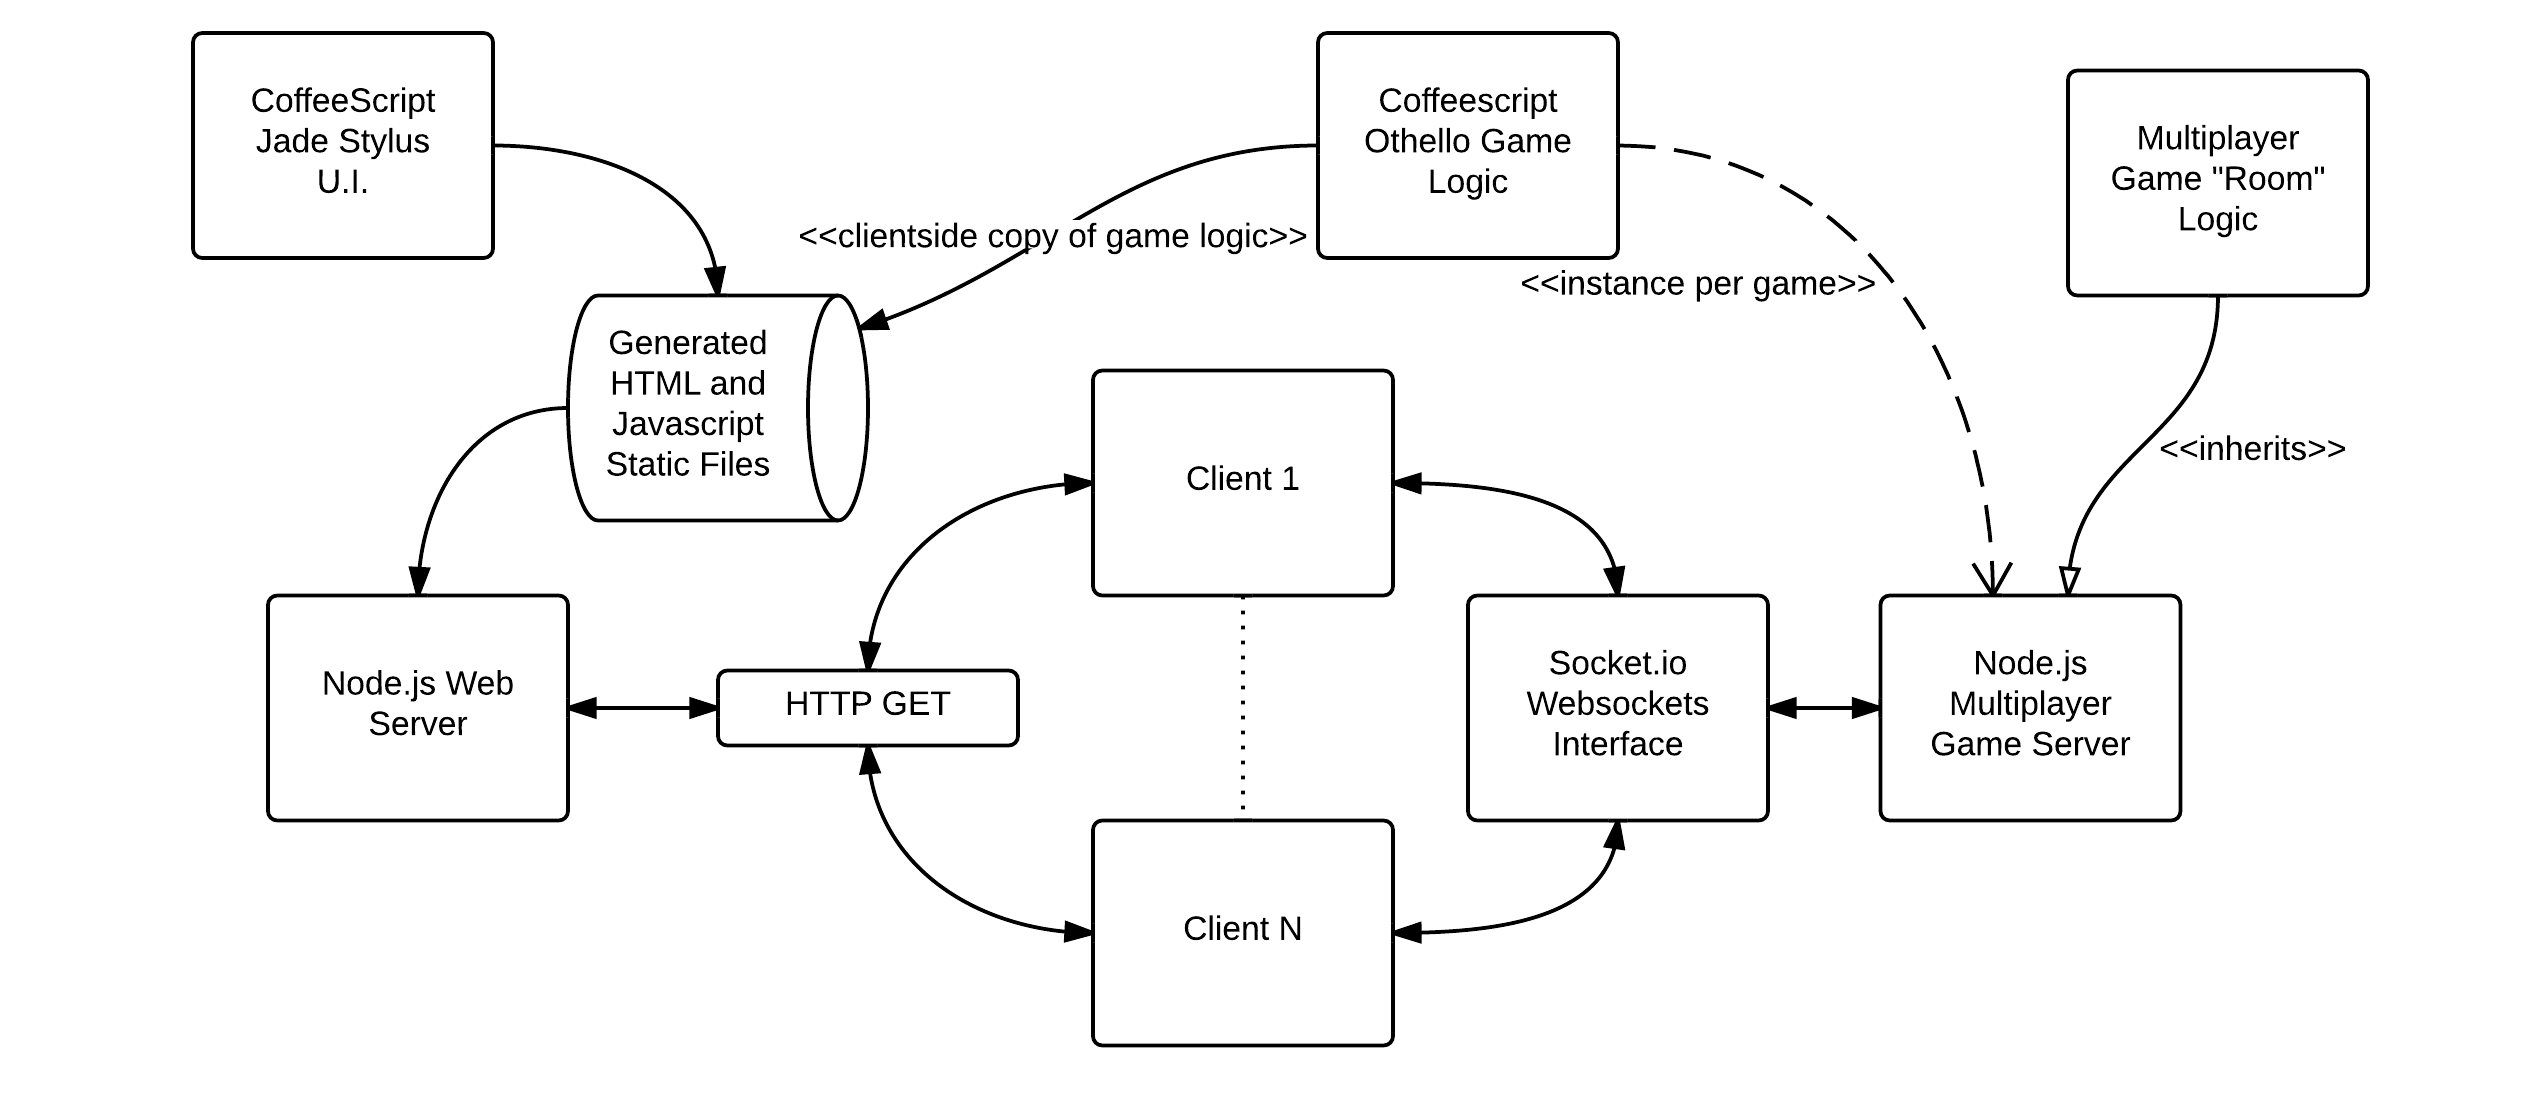
\includegraphics[width=\textwidth]{SoftwareEngineering.png}

\section{Testing}
In accordance with Test Driven Development principles, one of the first stages around building the project was to produce a comprehensive test framework, which could be used throughout the project to ensure that the behaviour of the system, and its components, are correct. To do this, we have utilised the Jasmine Javascript testing framework, with the jasmine-node module such that we can quickly write tests and maintain the core behaviour when we add extra features to the design.

\begin{verbatim}
C:\Code\othello>jasmine-node --coffee --matchall test
............................

Finished in 0.047 seconds
28 tests, 42 assertions, 0 failures
\end{verbatim}

\section{Designing the Othello Game}

The Othello game logic is relatively simple, but we worked in a top-down style to design the classes. We first considered how to build a console interface to the game class, and what sort of IO should be available to play the game. The requirements for this class was:
\begin{itemize}
\item Notifying the player who's turn to play it is, or notifications that there are no valid moves and that a player is being skipped.
\item Playing a move, given a move is valid
\item Outputting the score of the game.
\item Telling the players that the game has finished.
\end{itemize}
Whilst building these methods, we produced a list of requirements for the Othello Game class, which were:
\begin{itemize}
\item Constructor, to initialising the game to a default state given a board size.
\item A method returning a boolean if the game has finished or not.
\item An iterator, to recurse over each row and column of the board, returning the value of what is there such that it can be displayed.
\end{itemize}
Using this same principle, we recursively abstracted into the game logic, eventually producing a design that equates to the following diagram:

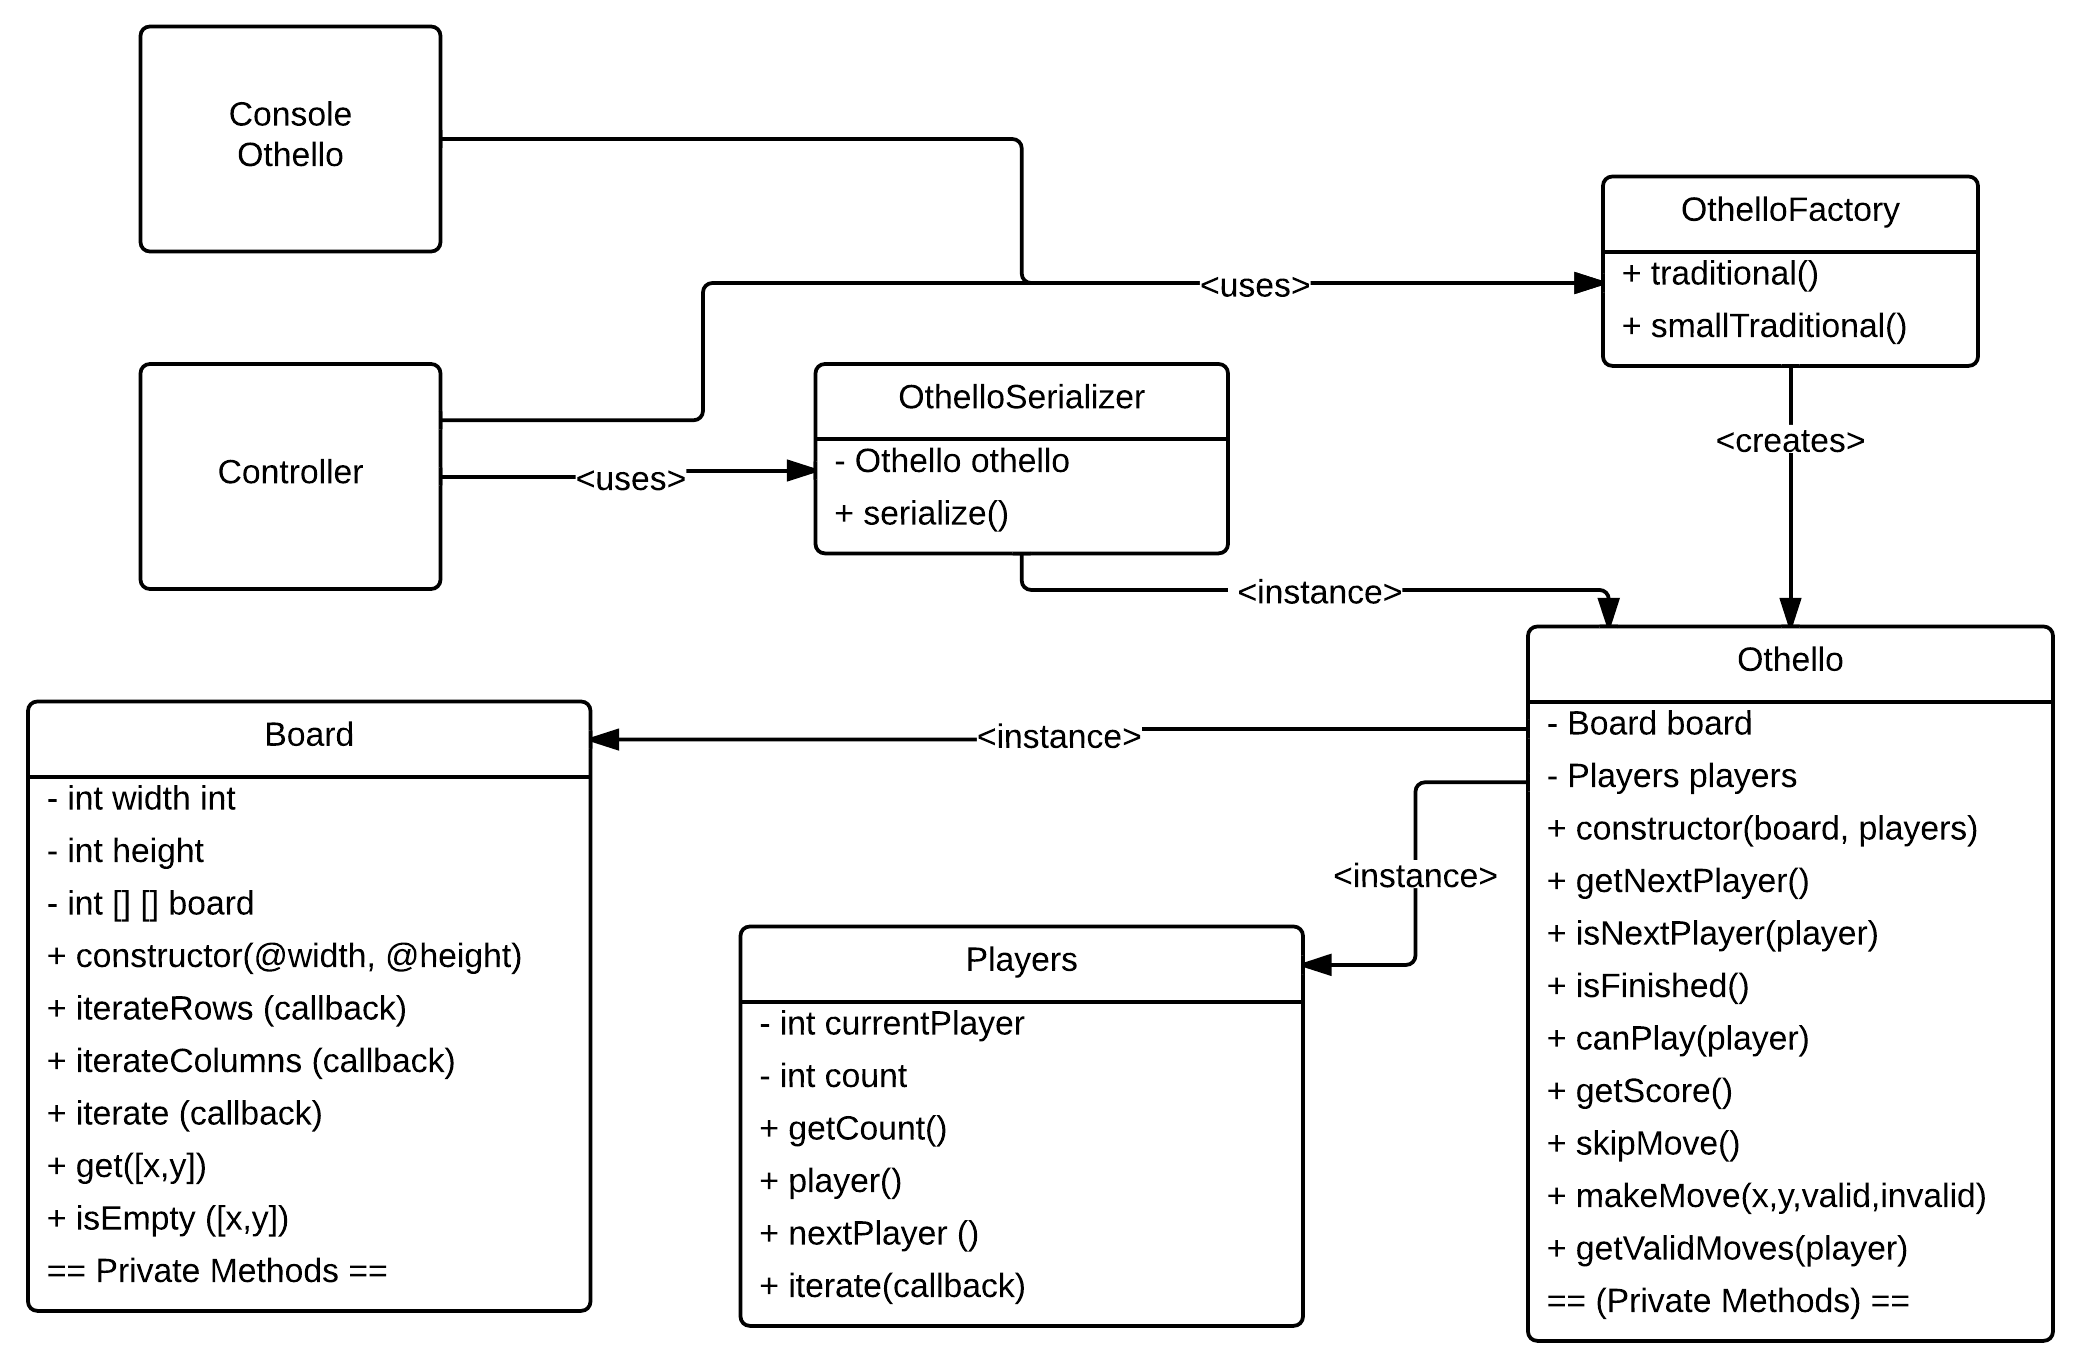
\includegraphics[width=\textwidth]{OthelloGameClassDiagram.png}

Utilising this design has given us a multitude of advantages. The seperation of the board class allows us to store and transmit the updates to the game to clients in a succint format. The \texttt{adaptor} pattern also allows us to reproduce the game logic in our Node.js HTTP server in a lightweight manner, with no changes to the code needing to be made between the console version but for the implementation of the \texttt{TraditionalOthello} class.

The design pattern we use most often is the \texttt{Iterator} pattern. The reason for this is it allows us to abstract away from the internal representation of the memory at each stage of the object hierarchy. Doing this lowers the rigidity of the code, as no information about the representation matters for the game.

A further feature that we implemented was a \texttt{HistoryOthello} class, allowing players to replay the game and undo moves. This was implemented via the \texttt{Decorator} pattern, used to keep the game design free of the extra backage that implemented this feature internally would cause.

The console version can be viewed and played via the file \texttt{game/ConsoleOthello.coffee}. It is dependant on the \texttt{commander} module.

\begin{verbatim}
Michal(w),  where would you like to place next stone?
X:  7
Y:  4
You can't place your stone there!
Michal(w),  where would you like to place next stone?
X:  7
Y:  5
  0 1 2 3 4 5 6 7
0 w w w w w w w b
1 w w w w w w w b
2 w w w w w w w b
3 w w w w w w w b
4 w w w w w w w b
5 w w w w w w w w
6 w w w w w w w b
7 w w w w w w w b
Game has ended, final scores:
Michal: 57
Tom: 7
\end{verbatim}
\section{HTTP Server}

The next stage in the production of our gaming server was the design of networking logic, and implementation of a client side U.I. to play the game on, and challenge other players on the same web page.

To minimize the workload of producing a large game server, we have utilised the following web technologies:
\begin{itemize}
\item Coffeescript is used to write code in, which minimizes the length of the code to write significantly, and providing (an illusion of) traditional object oriented programming environment.
\item Node.js allows the entire website to be written in Coffeescript (javascript natively), which means that our client and server can share code more simply.
\item Express.js allows the web server to be split into more manageable sections: views, routes, static scripting files and external node modules.
\item JQuery and JQuery UI Libraries have reduced the workload on producing the lobby, reducing complex HTML operations into  a single javascript call
\item socket.io is an interface to web sockets that provides very simple listeners and emitters, written in the same way for both Node.js server and client. This is incredibly powerful, and reduces the networking code down immensely such that it is a very simple transformation between design and implementation.
\item Paper.js gives us a more powerful interface to the web canvas framework, allowing our Othello GUI code to be written more succintly, with clickable objects being supported natively via the listener callback pattern.
\end{itemize}

Producing the Web server was done in a slightly differerent way to the way we produced the console game. We first built a proof of concept of the socket.io framework - with a simple box that would send to the server and write a message on the console. 

After we had our proof of concept produced, we designed the network schematics for how we wanted the communication between clients and the server to roughly follow. The Lobby Connection flowchart is available below.

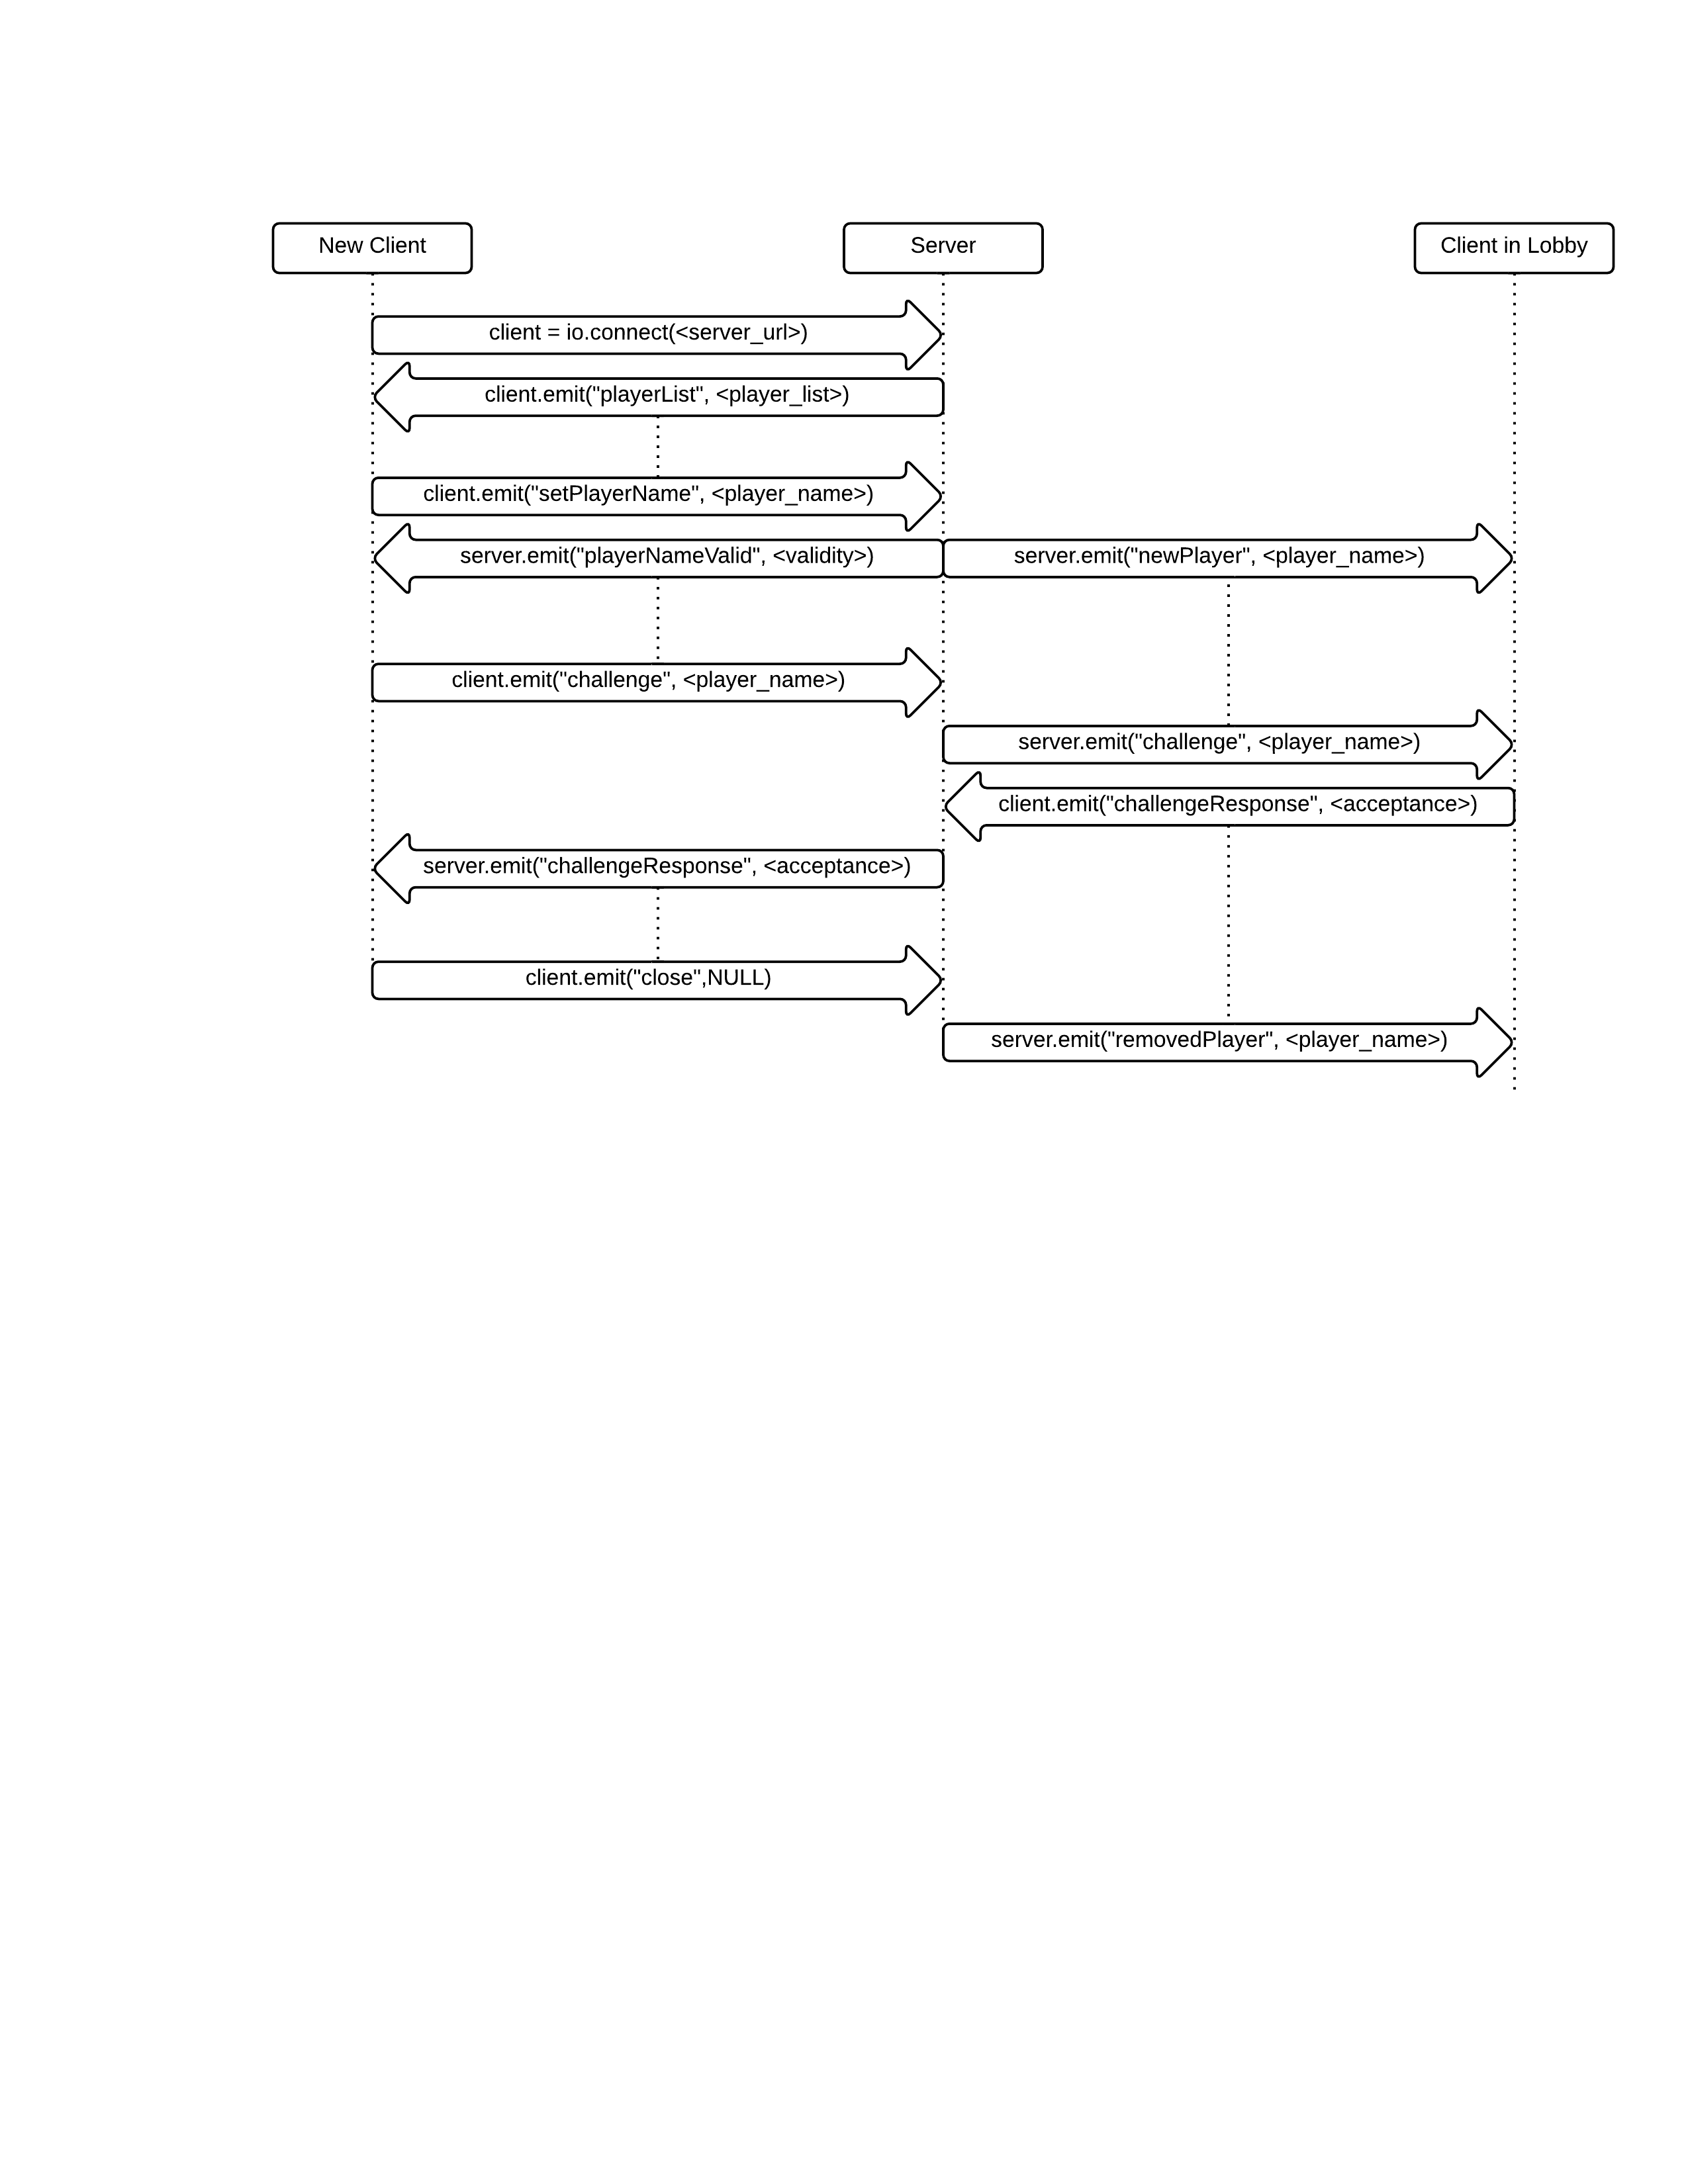
\includegraphics[width=\textwidth]{LobbyConnectionFlowchart.png}

Then, from this proof of concept we built upwards, iteratively improving until we had a full lobby backend. Alongside this work, we each played around with the various canvas libaries until we settled upon paper.js (the other contender was processing.js, but it required the entire screen to be redrawn for a small change). After the lobby was done, we used this same iterative improvement process on the GUI until we had our finished product.

\section{Conclusion}

For this coursework, we believe we have produced a simple design, which is easily extensible into differing applications.

We have ensured that what we have produced behaves correctly, via utilising the unit testing framework. 

We have ensured that our design is clear, through commenting our code as we have gone along

We have ensured that our design is scalable, via a split between HTTP servers and the websocket backend. The websocket backend is built in such a way that it could be easily scaled via a MapReduce style framework, simply splitting games and sockets between multiple servers.

We have ensured that we have a flexibility in our design, via multiple levels of abstraction away from internal representations of data. This means that our code is easily maintainable and extensible with minimal effort.

\section{Screenshot}

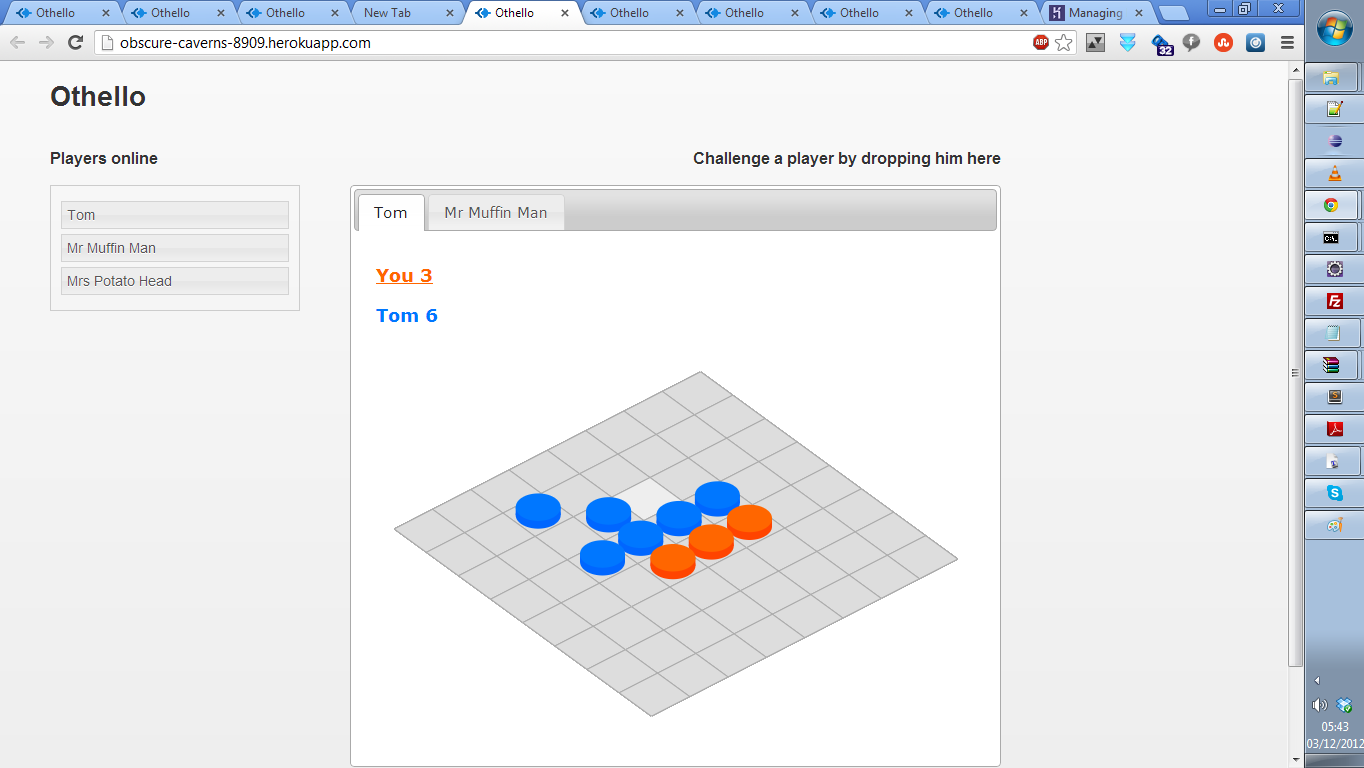
\includegraphics[width=\textwidth]{Screenshot.png}
\end{document}
